% SPEEDUPS
\newcommand{\meanspeedup}[0]{2.78x}

\startchapter{Migrating Legacy C Programs to a Streaming Representation}
\label{chap:profiling}

This chapter stands independently of the StreamIt project.  Rather
than starting with a stream programming language, we consider the
problem of starting with a legacy C application and migrating the code
to a streaming representation.  To address this problem, we equip the
programmer with a simple set of annotations (indicating possible
filter boundaries) and a dynamic analysis that tracks all
communication across those boundaries.  Our analysis outputs a stream
graph of the application as well as a set of macros for (unsoundly)
parallelizing the program and communicating the data needed.

Our analysis is unsound because it is based on a fixed set of dynamic
traces, rather than a conservative static analysis.  However, we argue
that this unsoundness enables us to provide programmers with more
information, that is ultimately more useful, than can be expected from
a static analysis.  We apply our methodology to six case studies,
including MPEG-2 decoding, MP3 decoding, GMTI radar processing, and
three SPEC benchmarks.  Our analysis extracts a useful block diagram
for each application, facilitating a translation to StreamIt and other
stream languages.  In addition, the parallelized versions run
correctly (given appropriate training inputs) and offer a
{\meanspeedup} mean speedup on a 4-core machine.

\section{Introduction}

While adopting a stream programming model is an attractive approach
for improving the performance of future applications, one of the
drawbacks of relying on a new programming model is that it does not
immediately address the vast quantities of legacy code that have
already been written in other languages.  There are 310 billion lines
of legacy code in industry today, and 75-80\% of the typical IT budget
is spent maintaining legacy systems~\cite{legacy}.  While much of this
code is amenable to streaming, the process of migrating the code to a
streaming representation is an arduous and time-consuming process.
The most important resources that could help with the translation --
such as the original author of the code, or the high-level design
documents that guided its implementation -- are often unavailable.
Thus, a fresh programmer is left with the daunting task of obtaining
an in-depth understanding of all the program modules, the dependences
between them, and the possibilities for safely extracting parallelism.

While there have been many efforts to automatically parallelize legacy
codes, few of them have focused on the pipeline parallelism that is
characteristic of the streaming domain.  It is even difficult to
express pipeline parallelism in a traditional programming model.  This
is in stark contrast to task parallelism, which is naturally supported
by threads, as well as data parallelism, which is supported by
dialects such as OpenMP.  The only efforts to exploit pipeline
parallelism in C programs have been very fine-grained, partitioning
individual instructions across processing
cores~\cite{ottoni05decoupled}.  Such fine-grained communication is
inefficient on commodity machines and demands new hardware
support~\cite{ottoni05decoupled,rangan04array}.  While a
coarse-grained partitioning is more desirable, it is difficult to
achieve at compile time due to the obscured data dependences in C;
constructs such as pointer arithmetic, function pointers, and circular
buffers (with modulo operations) make it nearly impossible to extract
coarse-grained parallelism from realistic C programs.

%Each pipeline stage can
%progress independently, so long as there is input data available from
%the previous stage.

%% Pipeline parallelism is an important abstraction, suitable to both new
%% and existing programs, that all parallel programmers should have at
%% their disposal.  Firstly, pipeline parallelism is often lurking in
%% otherwise sequential codes.  Loops with carried dependences can admit
%% a pipeline-parallel mapping (the dependence being carried by a single
%% pipeline stage) even though a data-parallel mapping is impossible.
%% Secondly, pipeline parallelism can be more efficient than data
%% parallelism due to improved instruction and data locality within each
%% pipeline stage, as well as point-to-point communication between cores
%% (there is no global scatter/gather).  Pipeline parallelism also offers
%% appeals over task parallelism, as all shared data can be communicated
%% in a deterministic producer/consumer style, eliminating the
%% possibility of data races.

In this chapter, we overcome the traditional barriers in exploiting
coarse-grained pipeline parallelism by embracing an {\it unsound}
program transformation.  Our key insight is that, for stream programs,
the data communicated across pipeline-parallel stages is stable
throughout the lifetime of the program.  No matter how obfuscated the
C implementation appears, the heart of the algorithm is following a
regular communication pattern.  For this reason, it is unnecessary to
undertake a heroic static analysis; we need only observe the
communication pattern at the beginning of execution, and then
``safely'' infer that it will remain constant throughout the rest of
execution (and perhaps other executions).

%then apply that pattern as the basis for
%parallelism in the remainder of the execution (and perhaps other
%executions).

As depicted in Figure~\ref{fig:overview}, our analysis does exactly
that.  We allow the programmer to naturally specify the boundaries of
pipeline partitions, and then we record all communication across those
boundaries during a training run.  The communication trace is emitted
as a stream graph that reflects the high-level structure of the
algorithm (aiding a possible translation to StreamIt), as well as a
list of producer/consumer statements that can be used to trace down
problematic dependences.  The programmer never needs to worry about
providing a ``correct'' partitioning; if there is no parallelism
between the suggested partitions, it will result in cycles in the
stream graph.  If the programmer is satisfied with the parallelism in
the graph, he recompiles the annotated program against a set of macros
that are emitted by our analysis tool.  These macros serve to fork
each partition into its own process and to communicate the recorded
locations using pipes between processes.

\begin{figure}[t]
%% \newlength{\myoffset}
%% \setlength{\myoffset}{-\textwidth}
%% \addtolength{\myoffset}{\columnwidth}
%% \hspace{\myoffset}
\hspace{-0.25in}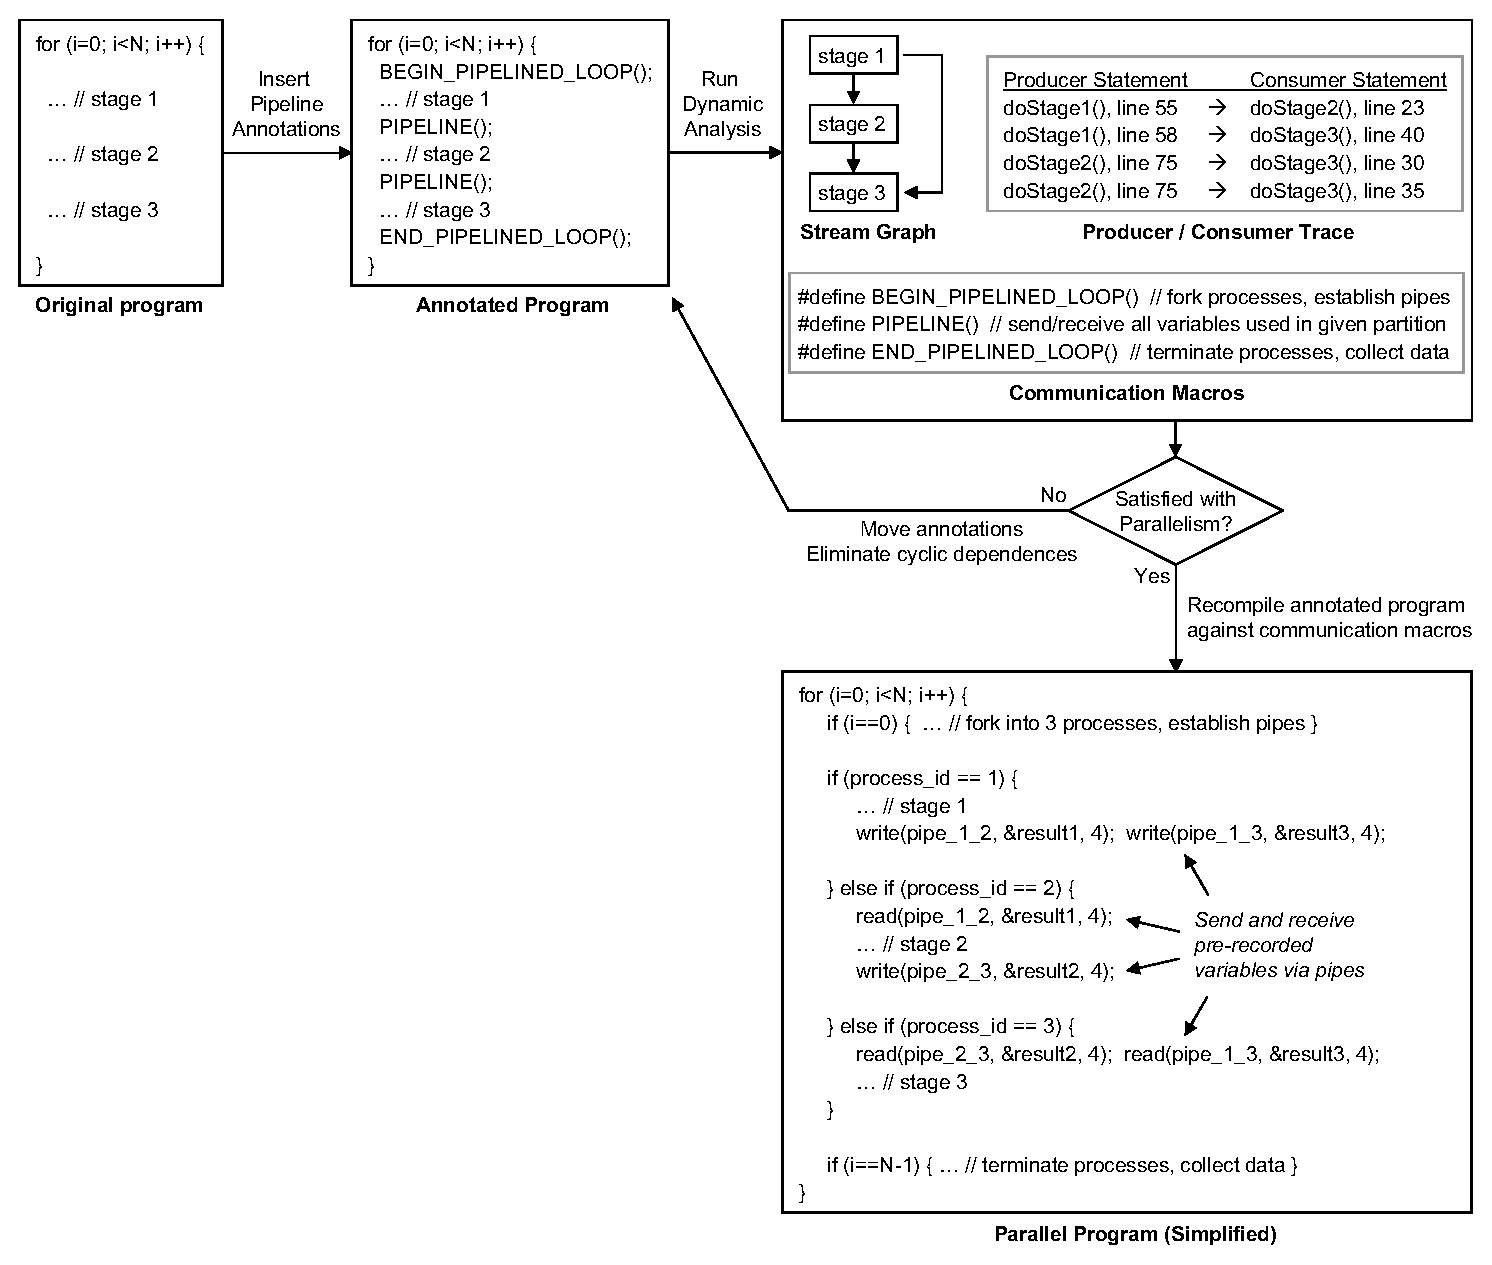
\psfig{file=profiling/intro-overview.eps,width=7in}
\vspace{-18pt}
\caption{Overview of our approach.\protect\label{fig:overview}}
\vspace{-6pt}
\end{figure}

Though our transformation is grossly unsound, we argue that it is
quite practical within the domain of streaming applications.  Because
pipeline parallelism is deterministic, any incorrect transformations
incurred by our technique can be identified via traditional testing
methods, and failed tests can be fixed by adding the corresponding
input to our training set.  Further, the communication trace provided
by our analysis is useful in aiding manual parallelization of the code
-- a process which, after all, is only sound insofar as the
programmer's understanding of the system.  By improving the
programmer's understanding, we are also improving the soundness of the
current best-practice for parallelizing legacy C applications.

We have applied our methodology to six case studies: MPEG-2 decoding,
MP3 decoding, GMTI radar processing, and three SPEC benchmarks.  Our
tool was effective at parallelizing the programs, providing a mean
speedup of {\meanspeedup} on a four-core architecture.  Despite the
potential unsoundness of the tool, our transformations correctly
decoded ten popular videos from YouTube, ten audio tracks from
MP3.com, and the complete test inputs for GMTI and SPEC benchmarks.
At the same time, we did identify specific combinations of training
and testing data (for MP3) that lead to erroneous results.  Thus, it
is important to maximize the coverage of the training set and to apply
the technique in concert with a rigorous testing framework.

The remainder of this chapter is organized as follows.  In
Section~\ref{sec:stability}, we show that stream programs have a
stable communication pattern.  Communication observed at the start of
execution is often preserved throughout the program lifetime, as well
as other executions.  Section~\ref{sec:workflow} describes our dynamic
analysis tool and programmer methodology to iteratively extract stream
parallelism from C programs.  Section~\ref{sec:parallelization}
describes the implementation of the tool using the Valgrind
infrastructure.  Section~\ref{sec:results} is devoted to our case
studies, including performance results and the experience gained
during parallelization.  The remaining sections present related work,
future work, and a chapter summary.

%% CONTRIBUTIONS
%%
%% \item We define a simple API for indicating potential pipeline
%%   parallelism in the program.  Comparable to threads for task
%%   parallelism or OpenMP for data parallelism, this API serves as a
%%   fundamental abstraction for pipeline parallelism
%%   (Section~\ref{sec:workflow}).
%%
%% \item We present a dynamic analysis tool, built on top of Valgrind,
%%   for tracking producer/consumer relationships between coarse-grained
%%   program partitions.  The tool outputs a stream graph of the
%%   application, which validates or refutes the parallelism suggested by
%%   the programmer.  It also provides a detailed statement-level trace
%%   and a set of macros for automatic parallelization
%%   (Sections~\ref{sec:workflow}-\ref{sec:parallelization}).
%%
%% \item We apply our methodology to six case studies, encompassing
%%   MPEG-2 decoding, MP3 decoding, GMTI radar processing, and three SPEC
%%   benchmarks.  We extract meaningful stream graphs of each
%%   application, and achieve a {\meanspeedup} mean speedup on a 4-core
%%   architecture (Section~\ref{sec:results}).

%% \begin{figure*}[t]
%% \begin{center}
%% \hspace{0pt}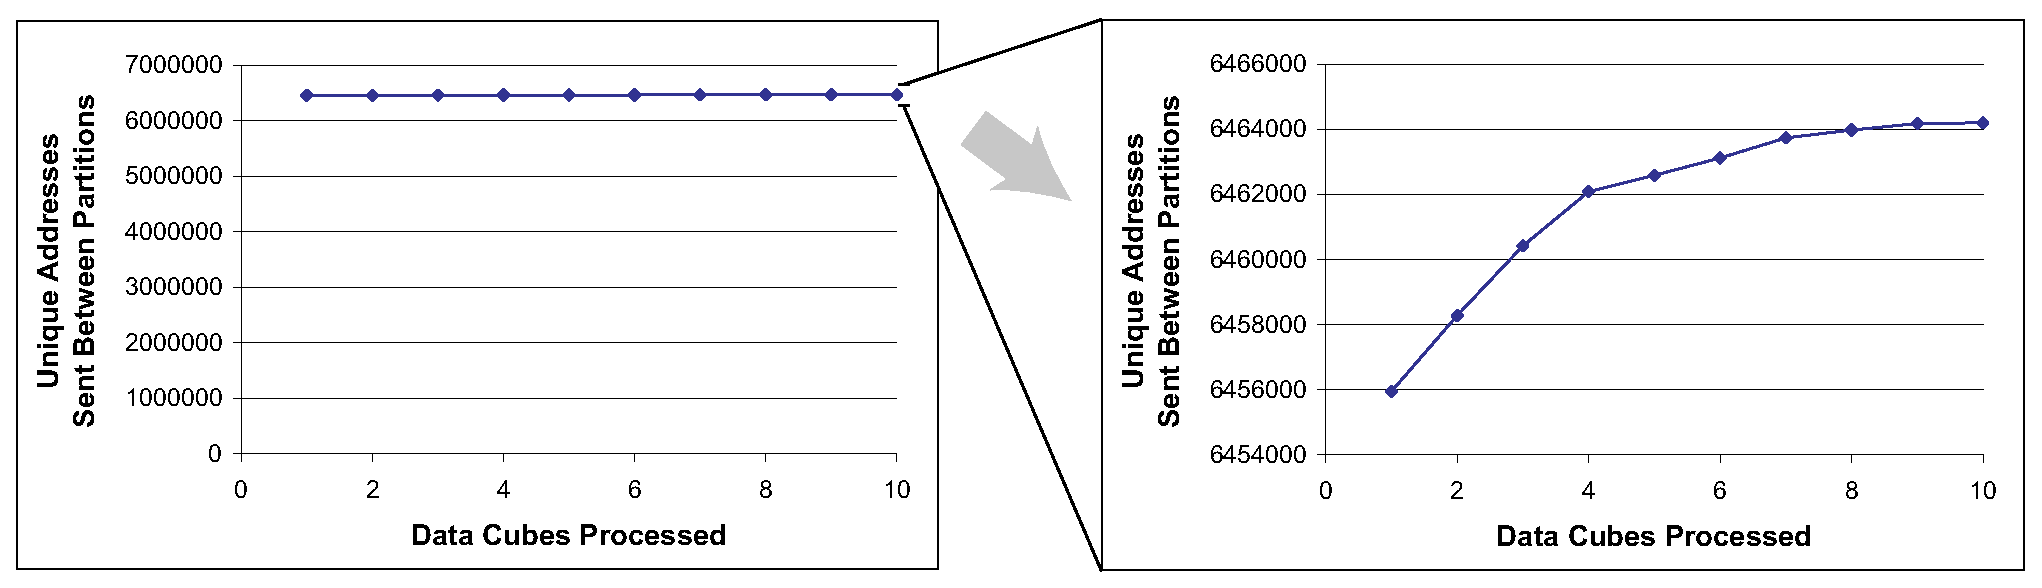
\psfig{file=profiling/gmti.eps,width=\textwidth}
%% \caption{Stability of streaming communication patterns for GMTI radar
%%   processing. See Figure~\ref{fig:gmti-graph} for a stream graph of
%%   the application.\protect\label{fig:gmti-stability}}
%% \end{center}
%% \end{figure*}

%% \begin{table*}[t]
%% \vspace{10pt}
%% \small
%% \begin{center}
%% \begin{tabular}{|l|l|l|l|}
%% \hline
%% {\bf Benchmark} & {\bf Training Input} & {\bf Testing Input} & {\bf Testing Output} \\ \hline
%% \parbox{0.8in}{~ \vspace{-3pt} \\ MPEG-2 \\ Decoding  ~\\ \vspace{-7pt}} &  First 10 frames of a local video & \parbox{1.9in}{~ \vspace{-3pt} \\ Top 10 short videos from YouTube\\ + user-supplied frame size ~ \\ \vspace{-7pt}} & 100\% correct\\ \hline
%% \parbox{0.8in}{~ \vspace{-3pt} \\ MP3 \\ Decoding  ~\\ \vspace{-7pt}} & First 3 samples of a local CD track & \parbox{1.9in}{~ \vspace{-3pt} \\ Top 10 downloads from mp3.com\\ (tens of thousands of samples) ~\\ \vspace{-7pt}} & 100\% correct \\ \hline
%% \parbox{0.8in}{~ \vspace{-3pt} \\ GMTI Radar \\ Processing  ~\\ \vspace{-7pt}} & \parbox{2in}{~ \vspace{-3pt} \\ First 10 data cubes of input + \\ user direction to fill sparse array ~\\ \vspace{-7pt}} & Rest of input (50 data cubes) & 100\% correct \\ \hline
%% \end{tabular}
%% \vspace{-6pt}

%% \caption{Stability of streaming communication patterns across
%%   different input files.  Using the tool and methodology described in
%%   this paper, we profiled the execution of three realistic streaming
%%   applications for a few iterations of a training input.  We used the
%%   observed communication trace to parallelize the program, executing
%%   each pipeline stage in a separate address space and relying on the
%%   trace to satisfy all of the data dependences.  Despite the short
%%   training period and the potential unsoundness of the technique, the
%%   trace was sufficiently stable to correctly execute unrelated input
%%   files (from YouTube and MP3.com) in a parallel
%%   context.\protect\label{tab:stability}}
%% \vspace{-6pt}
%% \end{center}
%% \end{table*}

\section{Stability of Stream Programs}
\label{sec:stability}

A dynamic analysis is most useful when the observed behavior is likely
to continue, both throughout the remainder of the current execution as
well as other executions (with other inputs).  Our hypothesis is that
stream programs exhibit very stable flows of data, enhancing the
reliability of dynamic analyses toward the point where they can be
trusted to validate otherwise-unsafe program transformations.  For the
purpose of our analysis, we consider a program to be {\it stable} if
there is a predictable set of memory dependences between pipeline
stages.  The boundaries between stages are specified by the programmer
using a simple set of annotations; the boundaries used for the
experiments in this section are illustrated by the stream graphs that
appear later (Figure~\ref{fig:mpeg2-mp3-graphs}).

\subsection*{Stability Within a Single Execution}

Our first experiment explores the stability of memory dependences
within a single program execution.  We profiled MPEG-2 and MP3
decoding using the most popular content from YouTube\footnote{YouTube
  videos were converted from Flash to MPEG-2 using ffmpeg and
  vixy.net.} and MP3.com; results appear in
Figures~\ref{fig:mpeg2-addresses} and~\ref{fig:mp3-addresses}.  These
graphs plot the cumulative number of unique addresses that are passed
between program partitions as execution proceeds.  The figures show
that after a few frames, the program has already performed a
communication for most of the addresses it will ever send between
pipeline stages.

In the case of MPEG-2, all of the address traces remain constant after
50 frames, and 8 out of 10 traces remain constant after 20 frames.
The videos converge at different rates in the beginning due to varying
parameters and frame types; for example, video 10 contains an
intra-coded frame where all other videos have a predictive-coded
frame, thereby delaying the use of predictive buffers in video 10.
Video 1 communicates more addresses than the others because it has a
larger frame size.

MP3 exhibits a similar stability property, though convergence is
slower for some audio tracks.  While half of the tracks exhibit their
complete communication pattern in the first 35 frames, the remaining
tracks exhibit a variable delay (up to 420 frames) in making the final
jump to the common communication envelope.  These jumps correspond to
elements of two parameter structures
% ({\tt III\_side\_info} and {\tt III\_scalefac}) 
which are toggled only upon encountering certain frame types.  Track
10 is an outlier because it starts with a few layer-1 frames, thus
delaying the primary (layer-3) communication and resulting in a higher
overall communication footprint.  The only other file to contain
layer-1 frames is track 9, resulting in a small address jump at
iteration 17,900 (not illustrated).

\begin{figure}[t]
\begin{minipage}{3.075in}
\hspace{-0.05in}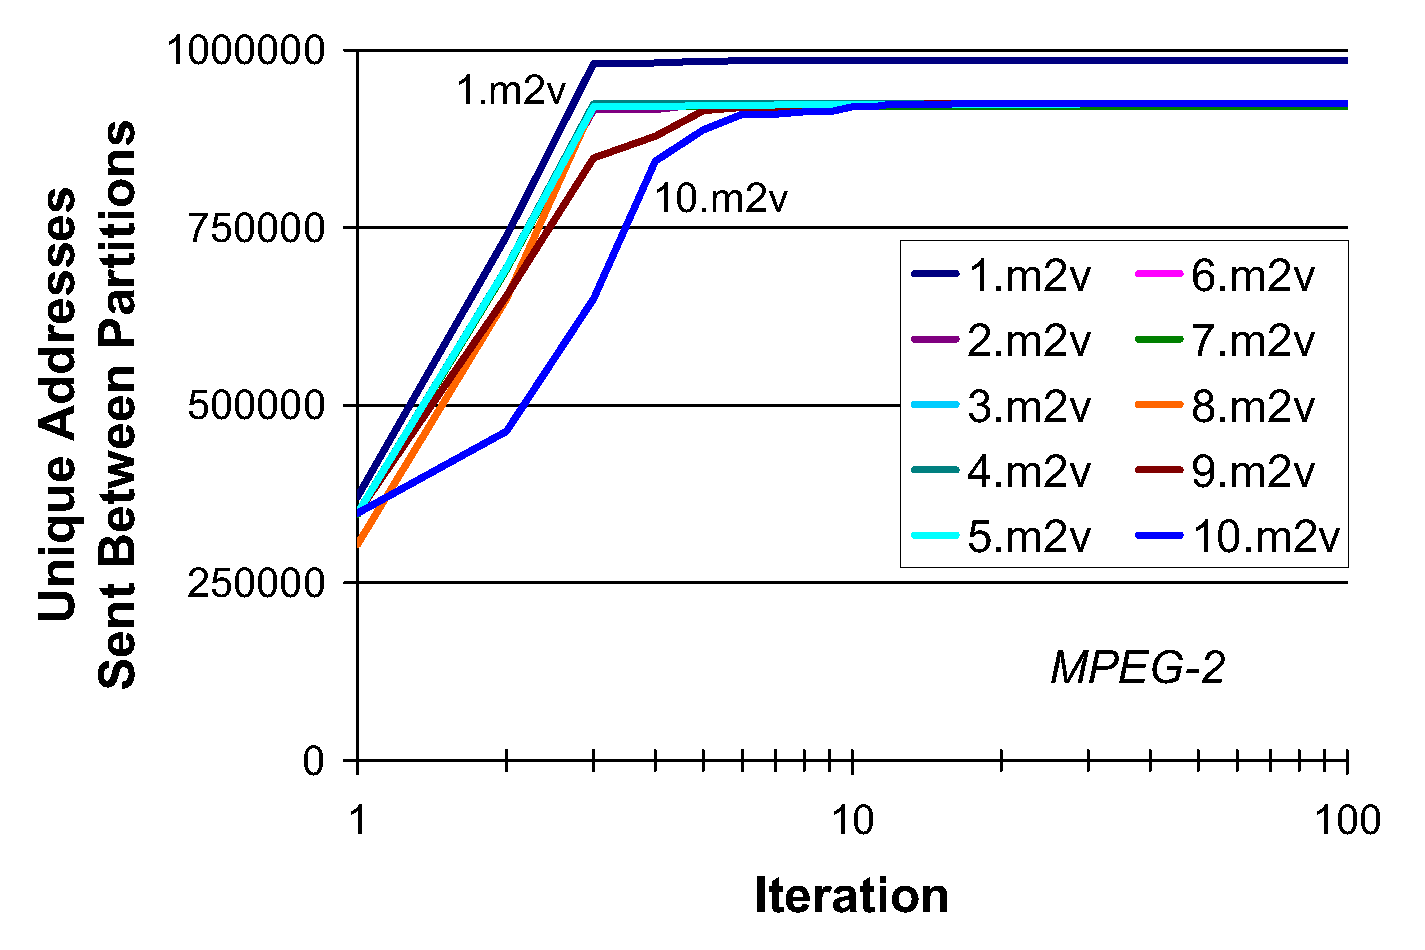
\psfig{file=profiling/mpeg2-addresses.eps,width=3.125in}
\vspace{-12pt}
\caption[Stability of streaming communication patterns for MPEG-2
  decoding.]{Stability of streaming communication patterns for MPEG-2
  decoding.  The decoder was monitored while processing the top 10
  short videos
% (25-35 seconds) 
from YouTube.  See Figure~\ref{fig:mpeg2-mp3-graphs}a for a stream
graph of the application.\protect\label{fig:mpeg2-addresses}}
\end{minipage}
\hspace{0.3in}
\begin{minipage}{3.02in}
\hspace{-0.05in}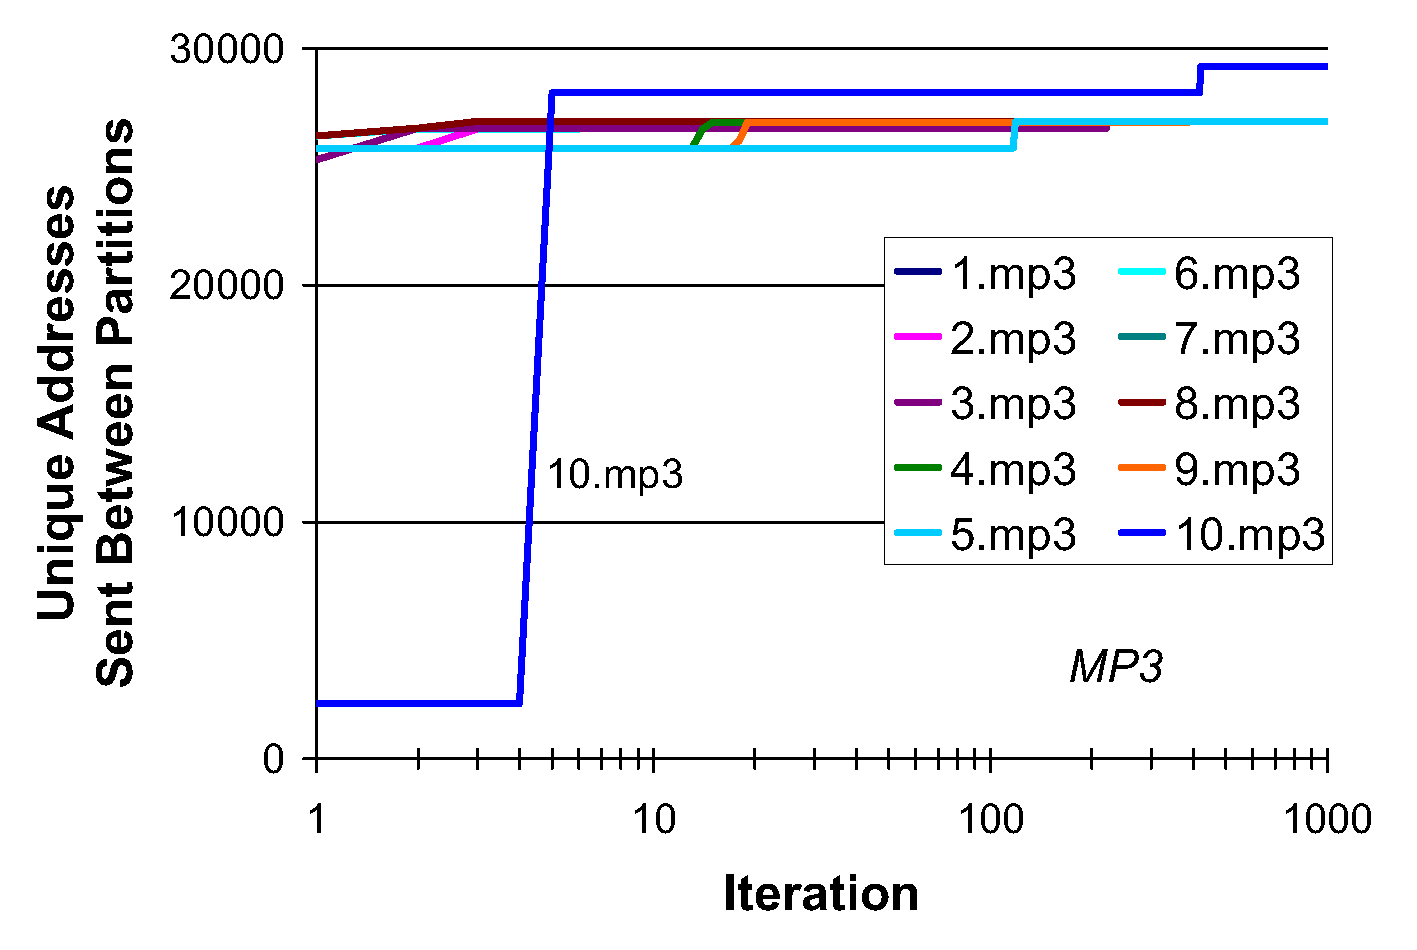
\psfig{file=profiling/mp3-addresses.eps,width=3.125in}
\vspace{-12pt}
\caption[Stability of streaming communication patterns for MP3
  decoding.]{Stability of streaming communication patterns for MP3
  decoding.  The decoder was monitored while processing the top 10
  tracks from MP3.com.  See Figure~\ref{fig:mpeg2-mp3-graphs}b for a
  stream graph of the application.  \protect\label{fig:mp3-addresses}}
\end{minipage}
\end{figure}

\begin{figure}[t]
\begin{minipage}{3.075in}

\psfig{file=profiling/mpeg2-matrix.eps,width=3.07in}
\vspace{-12pt}
\caption[Training needed for correct parallelization of
  MPEG-2.]{Minimum number of training iterations (frames) needed on
  each video in order to correctly decode the other videos.
  \protect\label{tab:mpeg2-matrix}}
\end{minipage}
\hspace{0.3in}
\begin{minipage}{3.02in}

\psfig{file=profiling/mp3-matrix.eps,width=3.07in}
\vspace{-12pt}
\caption[Training needed for correct parallelization of MP3.]{Minimum
  number of training iterations (frames) needed on each track in order
  to correctly decode the other tracks.
  \protect\label{tab:mp3-matrix}}
\end{minipage}
\end{figure}

It is important to note that there does exist a dynamic component to
these applications; however, the dynamism is contained within a single
pipeline stage.  For example, in MP3, there is a Huffman decoding step
that relies on a dynamically-allocated lookup tree.  Throughout the
program, the shape of the tree grows and shrinks and is manipulated on
the heap.  Using a static analysis, it is difficult to contain the
effects of such dynamic data structures; a conservative pointer or
shape analysis may conclude that the dynamism extends throughout the
entire program.  However, using a dynamic analysis, we are able to
observe the actual flow of data, ignoring the intra-node communication
and extracting the regular patterns that exist between partitions.

%% We also tracked the communication pattern for the GMTI radar tracker
%% for the single input included in its distribution (see
%% Figure~\ref{fig:gmti-stability}).  Unlike MP3 and MPEG-2, GMTI has a
%% slow and gradual increase in the data communicated across iterations.
%% The user of our tool inspected the addresses that were increasing and
%% found that an array was being read in a sparse pattern that was
%% gradually encompassing the entire data space.  Based on this
%% knowledge, the programmer instructed the tool to communicate the
%% entire array between partitions for the sake of the program
%% transformations.

%% The stability observed here could prove useful when doing a dynamic
%% optimization of streaming applications.  By profiling only the first
%% few iterations, one can observe the bulk of the data dependences
%% present in later iterations.

%While the outlying cases and lingering
%addresses may be important to catch, they may also be expendable, as
%we describe next.

\subsection*{Stability Across Different Executions}

The communication patterns observed while decoding one input file can
often extend to other inputs as well.  Figures \ref{tab:mpeg2-matrix}
and~\ref{tab:mp3-matrix} illustrate the minimum number iterations
(i.e., frames) that need to be profiled from one file in order to
enable correct parallel decoding of the other files.  In most cases, a
training set of five loop iterations is sufficient to infer an address
trace that correctly decodes the other inputs in their entirety.  The
exceptions are tracks 9 and 10 of MP3 decoding, which are the only two
files containing layer-1 frames; because they execute code that is
never reached by the other files, training on the other files is
insufficient to expose the full communication trace.  In addition,
track 9 is insufficient training for track 10, as the latter contains
an early CRC error that triggers a unique recovery procedure.  As each
of these hazards is caused by executing code that is untouched by the
training set, the runtime system could easily detect such cases (using
guards around untrained code) and revert to a sequential execution for
the iterations in question.  Rigorous testing practices that
incorporate code coverage metrics would also help to reduce the risk
of encountering unfamiliar code at runtime.

The ability to generalize short training runs across multiple
executions relies on two aspects of our methodology.  First, as
described later, we require the user to supply a symbolic size for
each dynamically-allocated variable; this allows MPEG-2 address traces
to apply across different frame sizes.  Second, we coarsen the
granularity of the trace to treat structure types and
dynamically-allocated segments as atomic units.  That is, whenever a
single element of such a structure is communicated between partitions,
the rest of the structure is communicated as well (so long as it does
not conflict with a local change in the target partition).  Such
coarsening increases the tolerance to small element-wise changes as
observed in later iterations of MPEG-2 and MP3.  However, it does not
trivialize the overall result, as coarsening is only needed for a
small fraction of communicated addresses (15\% for MP3 and dependent
on frame size for MPEG-2).
% to make this statement stronger, should actually measure the
% percentage of communicated VARIABLES, though I could not gather this
% number for MPEG-2 at the last minute.  (For large frame sizes, 97%
% of the data is malloc'd.)

% details:
% we need coarsening for: III_scalefac, III_side_info, and possibly (?) info
% we do not need for:
% ch, fr_ps, gr, hybridIn, hybridOut, is, pcm_sample, ro, sb, stereo
% 
% fr_ps is a struct but it would just as well not be, so not counting
% many more variables COULD have been communicated, but only these were

While we have focused on MPEG-2 and MP3 in this section, we observe
similar stability across our other benchmarks (GMTI, bzip2, parser,
and hmmer).  As described in Section~\ref{sec:results}, we profile
five iterations of a training file and (with minimal programmer
intervention) apply the trace to correctly execute a test file.

\section{Migration Methodology}
\label{sec:workflow}

We introduce a dynamic analysis tool that empowers the programmer in
migrating legacy C applications to a streaming representation.  Using
this tool, the programmer follows the workflow illustrated in
Figure~\ref{fig:overview}.  The first step is to identify the main
loop in the application, which is typically iterating over frames,
packets, or another long-running data source.  The programmer
annotates the start and end of this loop, as well as the boundaries
between the desired pipeline-parallel partitions.  The tool reports
the percentage of execution time spent in each pipeline stage in order
to help guide the placement of pipeline boundaries.

In our current implementation, there are some restrictions on the
placement of the partition boundaries.  All boundaries must appear
within the loop body itself, rather than within a nested loop, within
nested control flow, or as part of another function (this is an
artifact of using macros to implement the parallelism).  The
programmer may work around these restrictions by performing loop
distribution or function inlining.  Also, though both {\tt for} loops
and {\tt while} loops are supported, there cannot be any {\tt break}
or {\tt continue} statements within the loop; such statements
implicitly alter the control flow in all of the partitions, an effect
that is difficult to trace in our dynamic analysis.  If such
statements appear in the original code, the programmer needs to
convert them to a series of {\tt if} statements, which our tool will
properly handle.

Once a loop has been annotated with partition boundaries, the
programmer selects a set of training inputs and runs our dynamic
analysis to trace the communication pattern.  The tool outputs a
stream graph, a list of producer/consumer statements, and a set of
communication macros for automatically running the code in parallel.

\begin{figure}[t!]
\centering
% 338 pix wide
\hspace{0in}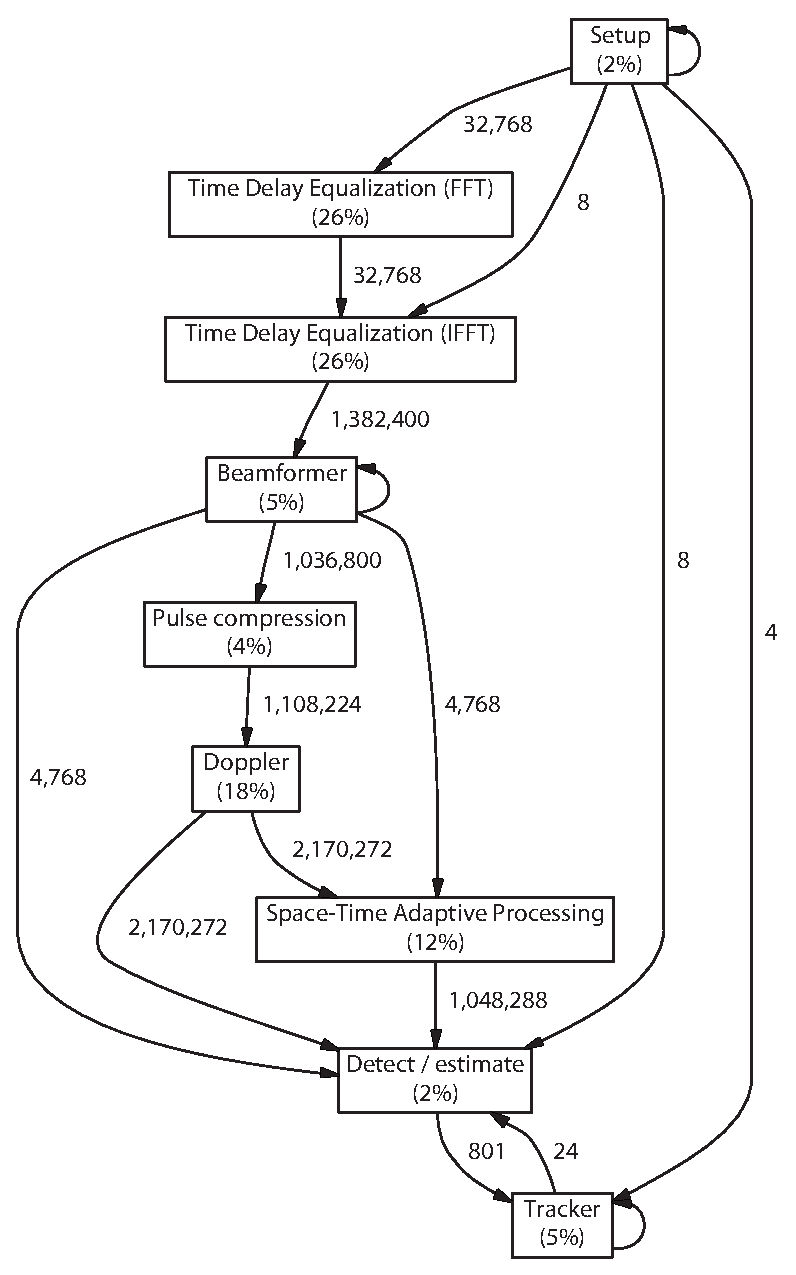
\psfig{file=profiling/gmti-opt.eps,width=2.9in}
\caption[Stream graph for GMTI, as extracted using our tool.]{Stream
  graph for GMTI, as extracted using our tool.  Nodes are annotated
  with their computation requirements, and edges are labeled with the
  number of bytes transferred per steady-state
  iteration.\protect\label{fig:gmti-graph-tool}}
\end{figure}

\begin{figure}[t!]
% to fill up this page
\vspace{6pt}
\centering
\hspace{0in}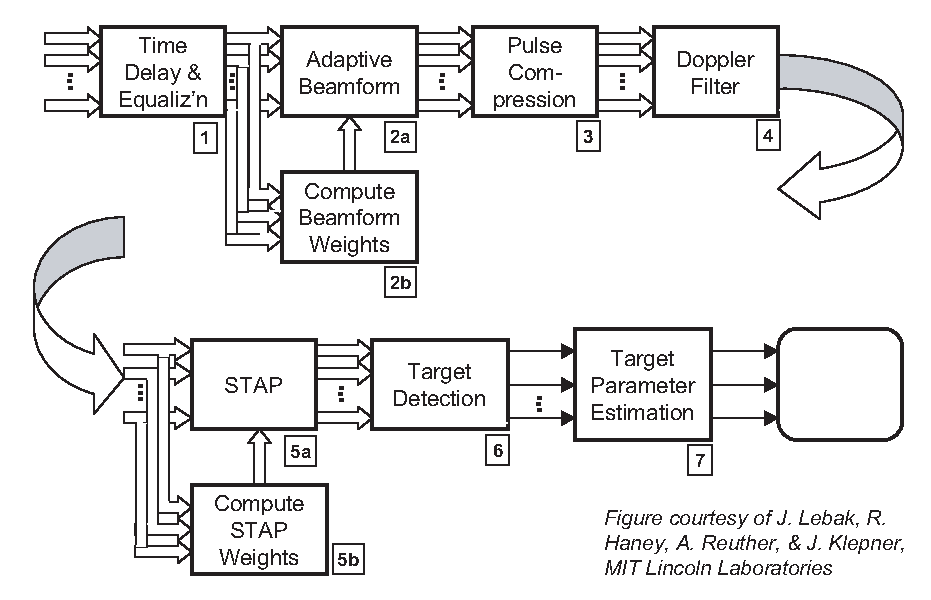
\psfig{file=profiling/gmti-spec.eps,width=3.3in}
\caption[Stream graph for GMTI, as it appears in the GMTI
  specification.]{Stream graph for GMTI, as it appears in the GMTI
  specification~\protect\cite{reuther03gmti}.\protect\label{fig:gmti-graph-spec}}
\vspace{-6pt}
\end{figure}

An example stream graph for GMTI radar processing appears in
Figure~\ref{fig:gmti-graph-tool}.  The graph extracted by our tool is
very similar to the block diagram from the GMTI specification, which
appears in Figure~\ref{fig:gmti-graph-spec}.  Our graph contains some
additional edges that are not depicted in the specification; these
represent communication of minor flags rather than the steady-state
dataflow.  Edges flowing from a node back unto itself (e.g., in Setup,
Beamformer, and Tracker) indicate mutable state that is retained
across iterations of the main loop.  Nodes without such dependences
are stateless with respect to the main loop, and the programmer may
choose to execute them in a data-parallel manner (see below).
% (There
%may also be more fine-grained data parallelism lurking in stateful
%nodes, due to nested loops within those nodes.)  
Overall, the tight correspondence between our extracted stream graph
and the original specification demonstrates that the tool can
effectively capture the underlying communication patterns, assisting
the programmer in understanding the opportunities and constraints for
parallelization.

Many nodes in a streaming application are suitable to data
parallelism, in which multiple loop iterations are processed in
parallel by separate instances of the node.  Such nodes are
immediately visible in the stream graph, as they lack a carried
dependence\footnote{In some cases, nodes with carried dependences on
  an outer loop can still be data-parallelized on an inner loop.  We
  perform such a transformation in MP3, though it is not fully
  automatic.} (i.e., a self-directed edge).  Our tool offers natural
support for exploiting data parallelism: the user simply provides an
extra argument to the {\tt PIPELINE} annotation, specifying the number
of ways that the following stage should be replicated (see
Figure~\ref{fig:data-parallelism}).  While this annotation does not
affect the profiler output, it is incorporated by the runtime system
to implement the intended parallelism.

Depending on the parallelism evident in the stream graph, it may be
desirable to iterate the parallelization process by adjusting the
pipeline partitions as well as the program itself.  The partitions can
execute in a pipeline-parallel manner so long as there are no cyclic
dependences between them.  If there are any strongly connected
components in the stream graph, they will execute sequentially; the
programmer can reduce the overhead by collapsing such partitions into
one.  Alternately, the programmer may be able to verify that certain
dependences can safely be ignored, in which case our analysis tool
will filter them out of future reports.  For example, successive calls
to malloc result in a data dependence that was originally reported by
our tool; however, this dependence (which stems from an update of a
memory allocation map) does not prohibit parallelism because the calls
can safely execute in any order.  Additional examples of non-binding
dependences include legacy debugging information such as timers,
counters, etc. that are not observable in the program output.
Sometimes, dependences can also be removed by eliminating the reuse of
certain storage locations (see Section~\ref{sec:results} for details).

\begin{figure}[t]
\centering
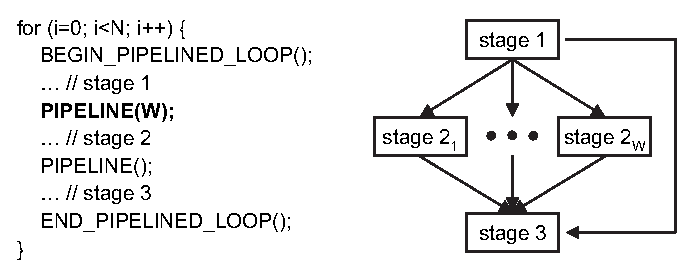
\psfig{file=profiling/data-parallelism.eps,width=3.5in}
\vspace{-6pt}
\caption[Specifying data parallelism.]{Programmers can specify data
  parallelism by passing an extra argument to the pipeline annotation.
  In this case, the runtime system executes W parallel copies of stage
  2.  \protect\label{fig:data-parallelism}}
\vspace{-6pt}
\end{figure}

Once the programmer is satisfied with the parallelism in the stream
graph, the code can automatically be executed in a pipeline-parallel
fashion using the communication macros emitted by the tool.  In most
cases, the macros communicate items from one partition to another
using the corresponding variable name (and potential offset, in the
case of arrays) from the program.  However, a current limitation is in
the case of dynamically-allocated data, where we have yet to automate
the discovery of variable name given the absolute addresses that are
communicated dynamically.  Thus, if the tool detects any communication
of dynamically-allocated data, it alerts the user and indicates the
line of the program that is performing the communication.  The user
needs to supply a symbolic expression for the name and size of the
allocated region.  Only two of our six benchmarks (MPEG-2 and bzip2)
communicate dynamically-allocated data across partition boundaries.
%Fortunately, in streaming applications, dynamically
%allocated data is rarely communicated across partitions, and when it
%is, the shape of the data is relatively simple (e.g., a video frame
%rather than a linked list).  
%
%It is also important to communicate the value of the pointer itself
%between processes, so that each process knows where to receive the
%dynamically allocated data.
%
%Though the frames have a dynamic size, a pointer to the frame is 
% held in a static variable that is easily supplied by the programmer.

\section{Implementation}
\label{sec:parallelization}

\subsection*{Dynamic Analysis Tool}

Our tool is built on top of Valgrind, a robust framework for dynamic
binary instrumentation~\cite{nethercote07valgrind}.  Our analysis
interprets every instruction of the program and (by tracing the line
number in the annotated loop) recognizes which partition it belongs
to.  The analysis maintains a table that indicates, for each memory
location, the identity of the partition (if any) that last wrote to
that location.  On encountering a store instruction, the analysis
records which partition is writing to the location.  Likewise, on
every load instruction, the analysis does a table lookup to determine
the partition that produced the value being consumed by the load.
Every unique producer-consumer relationship is recorded in a list that
is output at the end of the program, along with the stream graph and
communication macros.

There are some interesting consequences of tracking dependence
information in terms of load and store instructions.  In order to
track the flow of data through local variables, we disable register
allocation and other optimizations when preparing the application for
profiling.  However, as we do not model the dataflow through the
registers, the tool is unable to detect cases in which loaded values
are never used (and thus no dependence exists).  This pattern often
occurs for short or unaligned datatypes; even writes to such variables
can involve loads of neighboring bytes, as the entire word is loaded
for modification in the registers.  Our tool filters out such
dependences when they occur in parallel stack frames, i.e., a spurious
dependence between local variables of two neighboring function calls.
Future work could further improve the precision of our reported
dependences by also tracking dependences through registers (in the
style of Redux~\cite{nethercote03redux}).

As the dynamic analysis traces communication in terms of absolute
memory locations, some engineering was required to translate these
addresses to variable names in the generated macros.  (While absolute
addresses could also be used in the macros, they would not be robust
to changes in stack layout or in the face of re-compilation.)  We
accomplish this mapping using a set of gdb scripts\footnote{Our
  scripts rely on having compiled with debug information.}, which
provide the absolute location of every global variable as well as the
relative location of every local variable (we insert a known local
variable and print its location as a reference point).  In generating
the communication code, we express every address as an offset from the
first variable allocated at or below the given location.
%This transformation assumes that the program is memory safe, i.e., it
%does not depend on the relative layout of one variable versus another.
% --> actually some dependence is ok
In the case of dynamically-allocated data, the mapping from memory
location to variable name is not yet automated and requires programmer
assistance (as described in the previous section).

\subsection*{Parallel Runtime System}

The primary challenge in implementing pipeline parallelism is the need
to buffer data between execution stages.  In the sequential version of
the program, a given producer and consumer takes turns in accessing
the shared variables used for communication.  However, in the parallel
version, the producer is writing a given output while the producer is
still reading the previous one.  This demands that the producer and
consumer each have a private copy of the communicated data, so that
they can progress independently on different iterations of the
original loop.  Such a transformation is commonly referred to as
``double-buffering'', though we may wish to buffer more than two
copies to reduce the synchronization between pipeline stages.

There are two broad approaches for establishing a buffer between
pipeline stages: either explicitly modify the code to do the
buffering, or implicitly wrap the existing code in a virtual
environment that performs the buffering automatically.  The first
approach utilizes a shared address space and modifies the code for the
producer or consumer so that they access different locations; values
are copied from one location to the other at synchronization points.
Unfortunately, this approach requires a deep program analysis in order
to infer all of the variables and pointer references that need to be
remapped to shift the produced or consumed data to a new location.
Such an analysis seems largely intractable for a language such as C.

The second approach, and the one that we adopt, avoids the
complexities of modifying the code by simply forking the original
program into multiple processes.  The memory spaces of the processes
are isolated from one another, yet the processes share the exact same
data layout so no pointers or instructions need to be adjusted.  A
standard inter-process communication mechanism (such as pipes) is used
to send and buffer data from one process to another; a producer sends
its latest value for a given location, and the consumer reads that
value into the same location in its private address space.  At the end
of the loop's execution, all of the processes copy their modified data
(as recorded by our tool during the profiling stage) into a single
process that continues after the loop.  Our analysis also verifies
that there is no overlap in the addresses that are sent to a given
pipeline stage; such an overlap would render the program
non-deterministic and would likely lead to incorrect outputs.

\begin{table*}[t]
\begin{center}
{\tenpoint
\begin{tabular}{|l|l|l|l|}
\hline
{\bf Benchmark} & {\bf Description} & {\bf Source} & {\bf Lines of Code} \\ \hline \hline
MPEG-2 & MPEG-2 video decoder & MediaBench~\cite{lee97mediabench} & 10,000 \\ \hline
MP3 & MP3 audio decoder & Fraunhofer IIS~\cite{fraunhofer03mp3} & 5,000 \\ \hline
GMTI  & Ground Moving Target Indicator & MIT Lincoln Laboratory~\cite{reuther03gmti} & 37,000\\ \hline
197.parser & Grammatical parser of English language & SPECINT 2000 & 11,000 \\ \hline
256.bzip2 & bzip2 compression and decompression & SPECINT 2000 & 5,000 \\ \hline
456.hmmer & Calibrating HMMs for biosequence analysis & SPECCPU 2006 & 36,000 \\ \hline
\end{tabular}}
\caption{Benchmark characteristics.\protect\label{tab:prof-benchmarks}}
\end{center}
\end{table*}

% could add:
%  - for "backwards communication" (loop-carried, from later partition to earlier one), 
%    place the receive instruction at the bottom of the partition rather than the top

\section{Case Studies}
\label{sec:results}

To evaluate our approach, we applied our tool and methodology to six
realistic programs.  Three of these are traditional stream programs
(MPEG-2 decoding, MP3 decoding, GMTI radar processing) while three are
SPEC benchmarks (parser, bzip2, hmmer) that also exhibit regular flows
of data.  As illustrated in Table~\ref{tab:prof-benchmarks}, the size of
these benchmarks ranges from 5 KLOC to 37 KLOC.  Each program
processes a conceptually-unbounded stream of input data; our technique
adds pipeline parallelism to the toplevel loop of each application,
which is responsible for 100\% of the steady-state runtime.  (For
bzip2, there are two toplevel loops, one for compression and one for
decompression.)

In the rest of this section, we first describe our experience in
parallelizing the benchmarks before presenting performance results.

\subsection*{Parallelization Experience}

During the parallelization process, the programmer relied heavily on
the stream graphs extracted by our tool.  The final graphs for each
benchmark appear in Figures~\ref{fig:mpeg2-mp3-graphs}
and~\ref{fig:spec-graphs}.  In the graphs, node labels are gleaned
from function names and comments in the code, rather than from any
domain-specific knowledge of the algorithm.  Nodes are also annotated
with the amount of work they perform, while edges are labeled with the
number of bytes communicated per steady-state iteration.  Nodes that
were data-parallelized are annotated with their multiplicity; for
example, the Dequantize stage in MP3
(Figure~\ref{fig:mpeg2-mp3-graphs}b) is replicated twice.

As described in Section~\ref{sec:workflow}, our tool relies on some
programmer assistance to parallelize the code.  The manual steps
required for each benchmark are summarized in
Figure~\ref{fig:program-changes} and detailed in the following
sections.
% summarize comments about print statements here?

%% \begin{figure}[t]
%% \centering
%% \mbox{\hspace{0pt}}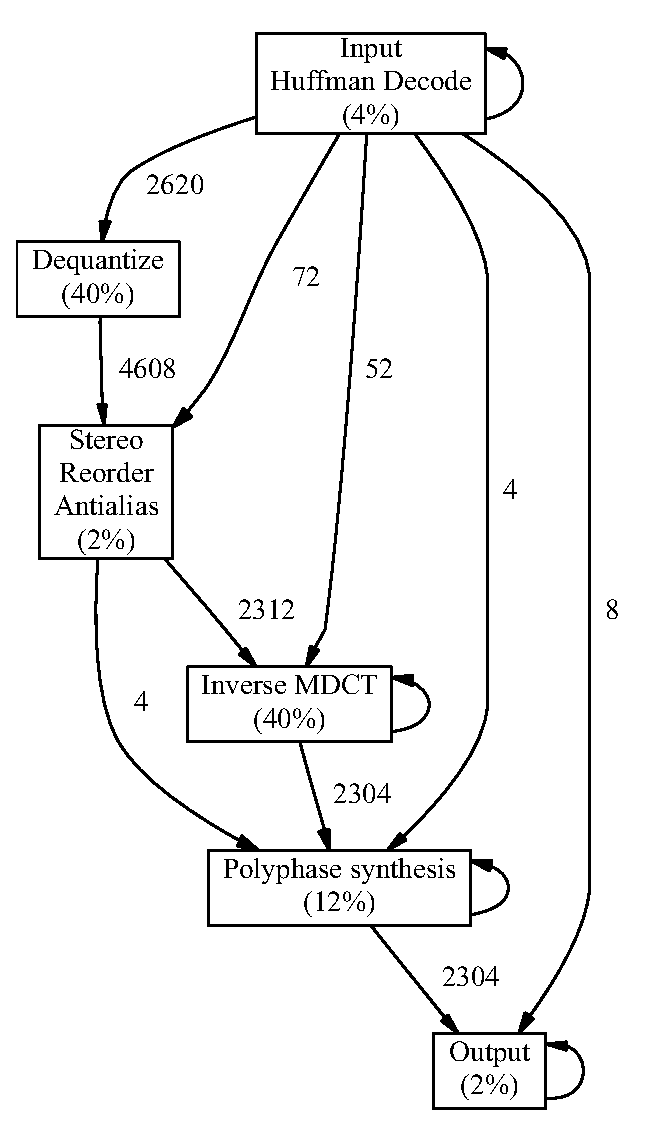
\psfig{file=profiling/mp3-orig.eps,width=1.93in}
%% \caption{Extracted stream graph for MP3 decoder.\protect\label{fig:mp3-graph}}
%% \end{figure}

%% The extracted graph is very similar to a block diagram for GMTI
%% (Figure~\ref{fig:gmti-graph}b) that is provided in the high-level
%% specification for the algorithm~\cite{reuther03gmti}.  By
%% automatically extracting an accurate high-level diagram of the
%% communication pattern, our analysis aids new programmers in
%% understanding and parallelizing the application.

%% \begin{figure}[t]
%% \vspace{-12pt}
%% \centering
%% % 454 pix wide
%% % seem to need the hspace command just to get it to center correctly
%% \hspace{0in}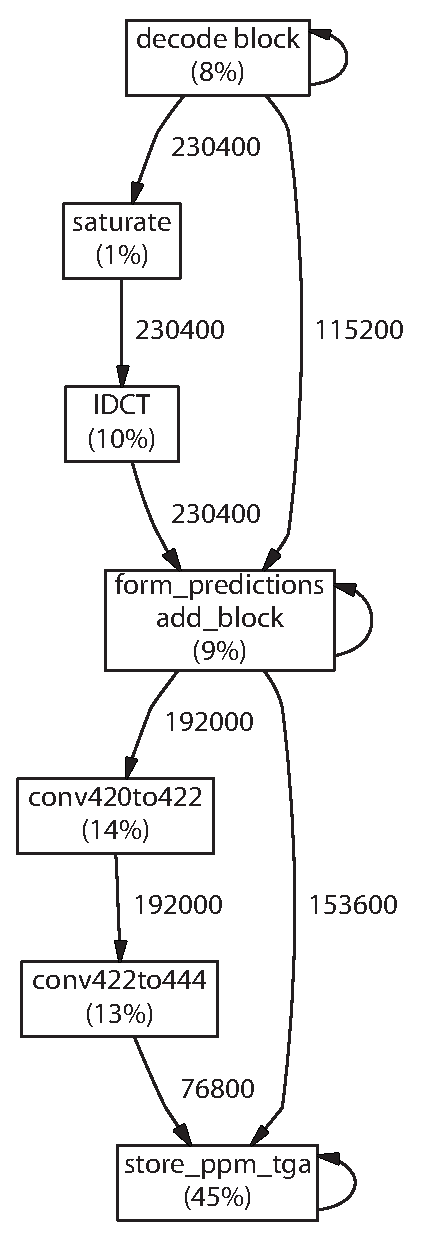
\psfig{file=profiling/mpeg2-opt.eps,width=1.52in}
%% \caption{Extracted stream graph for MPEG-2 decoder.  Nodes are
%%   numbered by their order of appearance in the sequential version of
%%   the code, and also labeled with the percentage of the program's
%%   work that they perform.  Edges are labeled with the number of bytes
%%   transferred per steady state
%%   iteration.\protect\label{fig:mpeg2-graph}}
%% \vspace{-12pt}
%% \end{figure}

\paragraph*{MPEG-2 Decoding} To obtain the stream graph for MPEG-2
(Figure~\ref{fig:mpeg2-mp3-graphs}a), the programmer iteratively
refined the program with the help of the dynamic analysis tool.
Because the desired partition boundaries fell in distinct functions,
those functions were inlined into the main loop.  Early return
statements in these functions led to unstructured control flow after
inlining; the programmer converted the control flow to if/else blocks
as required by our analysis.  The tool exposed an unintended data
dependence that was inhibiting parallelism: a global variable
(progressive\_frame) was being re-used as a temporary variable in one
module.  The programmer introduced a unique temporary variable for
this module, thereby restoring the parallelism.  In addition, the
updates to some counters in the main loop were reordered so as to
place them in the same pipeline stage that the counters were utilized.
%Finally, the programmer turned off an optional tracing flag to reduce
%the verbosity of print statements.  (Removed this because if it's
%optional, then that's just the version of the benchmark we used.)

\begin{figure}[t]
\centering
\vspace{-6pt}
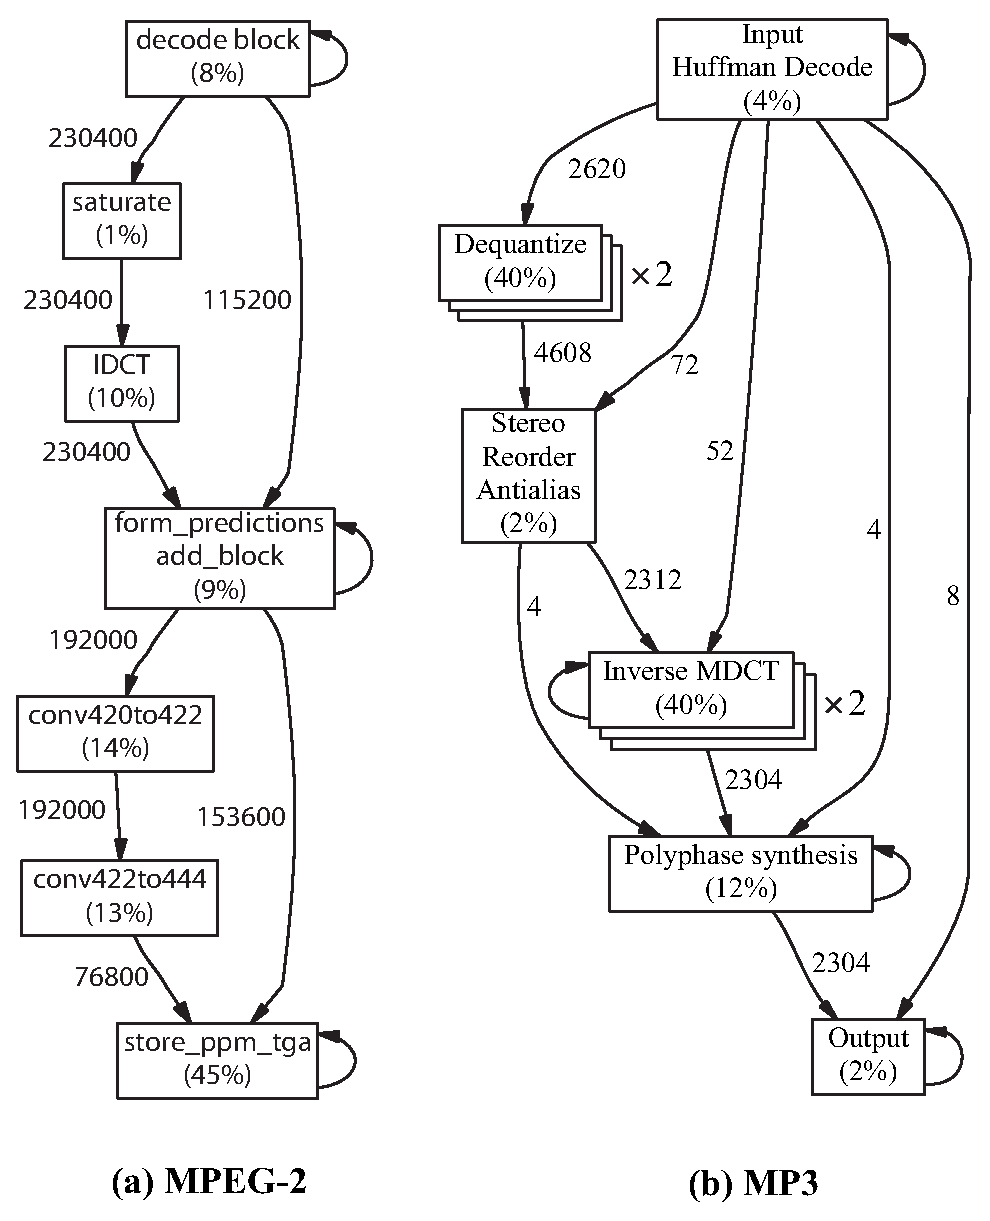
\psfig{file=profiling/mpeg2-mp3-graph.eps,width=3.5in}
\caption{Extracted stream graphs for MPEG-2 and MP3 decoding.\protect\label{fig:mpeg2-mp3-graphs}}
\vspace{-10pt}
\end{figure}

\begin{figure*}[t]
\centering
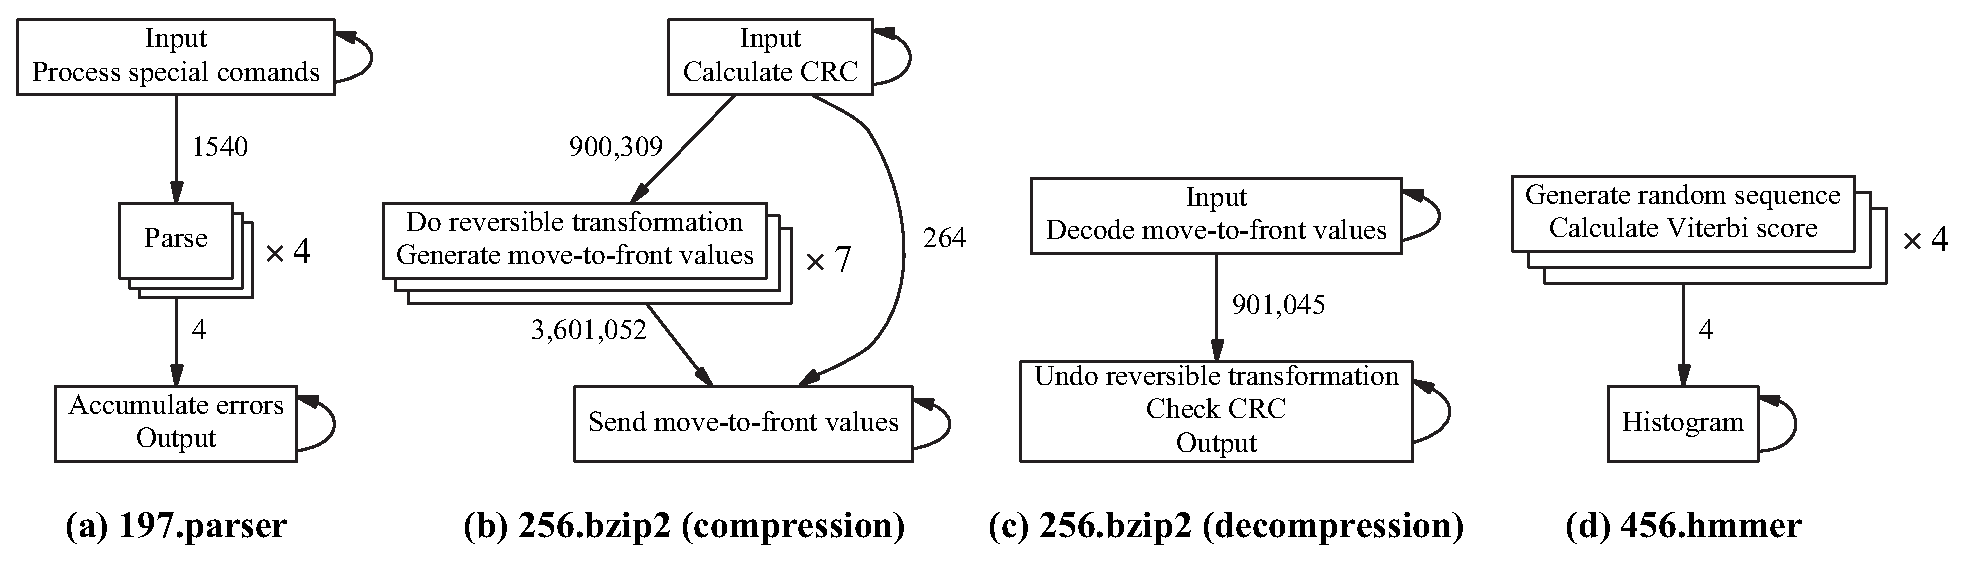
\psfig{file=profiling/spec-graphs.eps,width=\textwidth}
\caption[Extracted stream graphs for parser, bzip2, and
  hmmer.]{Extracted stream graphs for parser, bzip2 (compression and
  decompression) and hmmer.  \protect\label{fig:spec-graphs}}
\end{figure*}

In generating the parallel version, our tool required two
interventions from the programmer.  First, as the pipeline boundaries
spanned multiple loop nests, the communication code (auto-generated
for a single loop nest) was patched to ensure that matching send and
receive instructions executed the same number of times.  Second, as
described in Section~\ref{sec:workflow}, the programmer supplied the
name and size of dynamically-allocated variables (in this case, frame
buffers) that were sent between partitions.

\paragraph*{MP3 Decoding} The extracted stream graph for MP3 decoding
appears in Figure~\ref{fig:mpeg2-mp3-graphs}b.  In the process of
placing the pipeline boundaries, the programmer inlined functions,
unrolled two loops, and distributed a loop.  Four
dynamically-allocated arrays (of fixed size) were changed to use
static allocation, so that our tool could manage the communication
automatically.  As profiling indicated that the dequantization and
inverse MDCT stages were consuming most of the runtime, they were each
data-parallelized two ways.

In analyzing the parallelism of MP3, the programmer made three
deductions.  First, the initial iteration of the loop was found to
exhibit many excess dependences due to one-time initialization of
coefficient arrays; thus, the profiling and parallelization was
postponed to the second iteration.  Second, though the tool reports a
carried dependence in the inverse MDCT stage, the programmer found
that this dependence is on an outer loop and that it is safe to
data-parallelize the stage on an inner loop.  Finally, the programmer
judged the execution to be insensitive to the ordering of diagnostic
print statements, allowing the dependences between statements to be
ignored for the sake of parallelization.  (With some additional
effort, the original ordering of print statements can always be
preserved by extracting the print function into its own pipeline
stage.)

As in the case of MPEG-2, the programmer also patched the generated
communication code to handle nested loops.

\paragraph*{GMTI Radar Processing} The Ground Moving Target Indicator (GMTI)
is a radar processing application that extracts targets from raw radar
data~\cite{reuther03gmti}.  The stream graph extracted by our tool
(Figure~\ref{fig:gmti-graph-tool}) is very similar to the one that
appears in the GMTI specification (Figure~\ref{fig:gmti-graph-spec}).

%It performs adaptive,
%computationally-intensive filtering to minimize the impact of ground
%clutter and interference patterns.  
In analyzing GMTI, the programmer made minor changes to the original
application.  The programmer inlined two functions, removed the
application's self-timers, and scaled down an FFT window from 4096 to
512 during the profiling phase (the resulting communication code was
patched to transfer all 4096 elements during parallel execution).  

As print statements were judged to be independent of ordering, the
tool was instructed to ignore the corresponding dependences.
Dependences between calls to memory allocation functions (malloc/free)
were also disregarded so as to allow pipeline stages to manage their
local memories in parallel.  The programmer verified that regions
allocated within a stage remained private to that stage, thus ensuring
that the parallelism introduced could not cause any memory hazards.

Our tool reported an address trace that was gradually increasing over
time; closer inspection revealed that an array was being read in a
sparse pattern that was gradually encompassing the entire data space.
The programmer directed the tool to patch the parallel version so that
the entire array was communicated at once.

\begin{figure*}[t]
\hspace{-0.25in}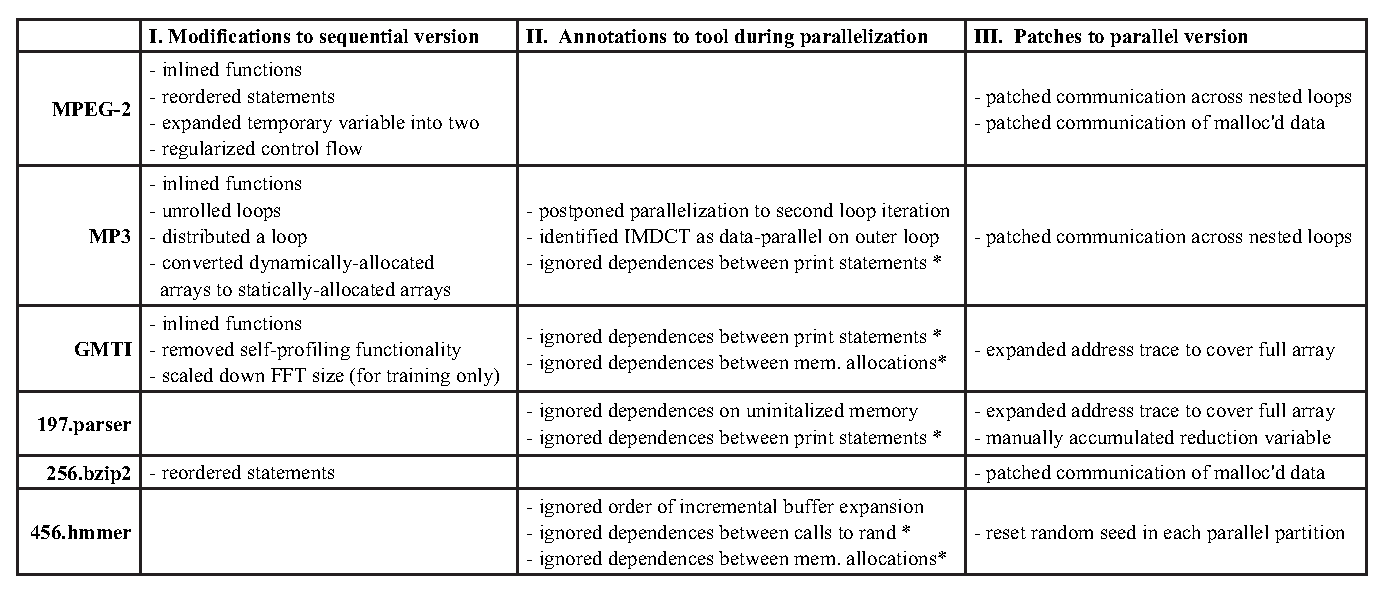
\psfig{file=profiling/program-changes.eps,width=7in}
\caption[Steps taken by programmer to assist with
  parallelization.]{Steps taken by the programmer to assist in
  parallelizing each benchmark.  Assistance may be needed to expose
  parallelism in the original code, to verify parallelism using the
  tool, or to handle special cases in the parallelized code.  Steps
  annotated with an asterisk (*) may change the observable behavior of
  the program\protect\footnotemark[1].
  \protect\label{fig:program-changes}}
\end{figure*}

%% \begin{figure}[t]
%% \centering
%% % seem to need the hspace command just to get it to center correctly
%% \hspace{0in}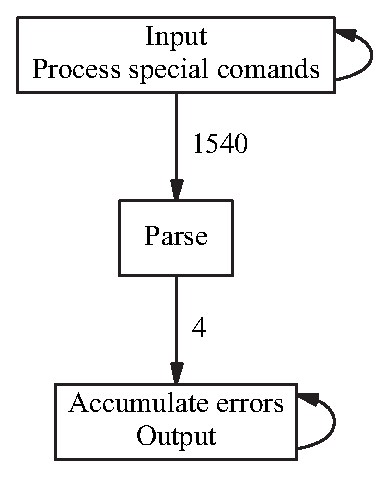
\psfig{file=profiling/parser-orig.eps,width=1.40in}
%% \caption{Original stream graph for 197.parser.  Edges are labeled with
%%   the number of bytes transferred per steady state iteration.  In the
%%   optimized graph (not shown), the Parse stage is duplicated four
%%   times.\protect\label{fig:parser-graph}}
%% \end{figure}

\paragraph*{Parser} The stream graph for 197.parser appears in
Figure~\ref{fig:spec-graphs}a.  Each steady-state iteration of the
graph parses a single sentence; the benchmark runs in batch mode,
repeatedly parsing all of the sentences in a file.  As indicated in
the graph, the cyclic dependences in the benchmark are limited to the
input stage (which performs file reading and adjusts the configuration
of the parser) and the output stage (which accumulates an error
count).  The parsing stage itself (which represents most of the
computation) retains no mutable state from one sentence to the next,
and can thus be replicated to operate on many sentences in parallel.
In our optimized version, the parsing stage is replicated four times.

During the iterative parallelization process, the programmer made
three adjustments to the program.  Our tool reported a number of
loop-carried dependences due to the program's implicit use of
uninitialized memory locations; the program allocates space for a
struct and later copies the struct (by value) before all of the
elements have been initialized.  This causes our tool to report a
dependence on the previous write to the uninitialized locations, even
though such writes were modifying a different data structure that has
since been de-allocated.  The programmer eliminated these dependence
reports by initializing all elements to a dummy value at the time of
allocation.

The programmer also made two adjustments to the communication trace
emitted by our tool.  One block of addresses was expanding gradually
over the first few iterations of the program.  Closer inspection
revealed that that sentences of increasing length were being passed
between partitions.  The programmer patched the trace to always
communicate the complete sentence buffer.
% (1500 characters)
Also, the programmer observed that in the case of errors, the parser's
error count needs to be communicated to the output stage and
accumulated there.  As none of our training or testing samples
elicited errors, our trace did not detect this dependence.

Our data-parallel version of the program may reorder the program's
print statements.  If desired, the print statements can be serialized
by moving them to the output stage.

%% \begin{figure}[t]
%% \centering
%% % seem to need the hspace command just to get it to center correctly
%% \hspace{0in}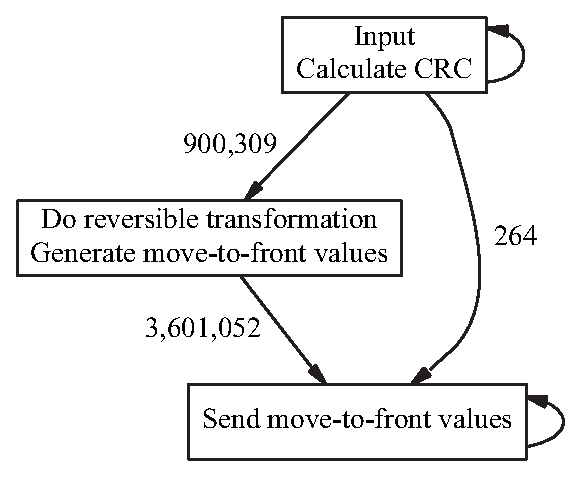
\psfig{file=profiling/bzip2-compress-orig.eps,width=2.15in}
%% \\{\bf (a) bzip2 compression}
%% \\ ~ \\ ~ \\
%% \hspace{0in}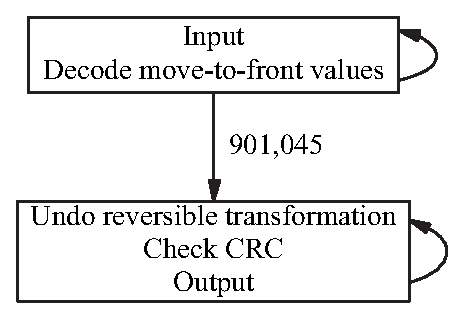
\psfig{file=profiling/bzip2-uncompress-orig.eps,width=1.69in}
%% \\{\bf (b) bzip2 decompression~~~}
%% \\ ~ 
%% \caption{Original stream graphs for 256.bzip2.  Edges are labeled with
%%   the number of bytes transferred per steady state iteration (at
%%   compression level 9).  In the optimized graph (not shown), the
%%   middle stage of the compression step (a) is duplicated seven
%%   times.\protect\label{fig:bzip2-graph}}
%% \vspace{-10pt}
%% \end{figure}

\paragraph*{Bzip2} The stream graphs for 256.bzip2 appear in
Figures~\ref{fig:spec-graphs}b and~\ref{fig:spec-graphs}c.  The
benchmark includes both a compression and decompression stage, which
were parallelized separately.

\footnotetext[1]{Reordering calls to malloc (or reordering calls to
  free) will only change the program's behavior if one of the calls
  fails.}

Because bzip2 compresses blocks of fixed size, the main compression
routine is completely data-parallel.  The only cyclic dependences in
the compressor are at the input stage (file reading, CRC calculation)
and output stage (file writing).  The programmer replicated the
compression stage seven ways to match the four-core machine; this
allows three cores to handle two compression stages each, while one
core handles a single compression stage as well as the input and
output stages.  The decompression step lacks data-parallelism because
the boundaries of the compressed blocks are unknown; however, it can
be split into a pipeline of two stages.

In parallelizing bzip2, the programmer reordered some statements to
improve the pipeline partitioning (the call to {\tt generateMTFValues}
moved from the output stage to the compute stage).  The programmer
also supplied the name and size of two dynamically-allocated arrays.

%This transfer represents a very coarse-grained communication: at
%compression level 9, the compression stage inputs and outputs a total
%of 4.5 MB of data per iteration.  Nonetheless, the compression stage
%exhibits a speedup of 3.07x; there is a 1.78x speedup for the
%decompression stage, and a 2.66x speedup for both stages combined.

%% \begin{figure}[t]
%% \centering
%% % seem to need the hspace command just to get it to center correctly
%% \hspace{0in}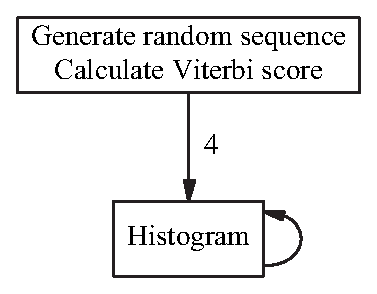
\psfig{file=profiling/hmmer-orig.eps,width=1.35in}
%% \caption{Original stream graph for 456.hmmer.  Edges are labeled with
%%   the number of bytes transferred per steady state iteration.  In the
%%   optimized graph (not shown), the top stage is duplicated four
%%   times.\protect\label{fig:hmmer-graph}}
%% \vspace{-10pt}
%% \end{figure}

\paragraph*{Hmmer} In 456.hmmer, a Hidden Markov Model is loaded at
initialization time, and then a series of random sequences are used to
calibrate the model.  Figure~\ref{fig:spec-graphs}d shows the
extracted stream graph for this benchmark.  The calibration is
completely data-parallel except for a histogram at the end of the
loop, which must be handled with pipeline parallelism.  In our
experiments, the programmer replicated the data-parallel stage four
ways to utilize the four-core machine.

Our tool reports three parallelism-limiting dependences for hmmer.
The first is due to random number generation: each iteration generates
a new random sample and modifies the random seed.  The programmer
chose to ignore this dependence, causing the output of our parallel
version to differ from the original version by 0.01\%.  Also, the
programmer made an important patch to the parallel code: after forking
from the original process, each parallel partition needs to set its
random seed to a different value.  Otherwise each partition would
follow an identical sequence of random values, and the parallel
program would sample only a fraction of the input space as the
original program.

The second problematic dependence is due to an incremental resizing of
an array to fit the length of the input sequence.  Since each parallel
partition can expand its own private array, this dependence is safely
ignored.  Finally, as in the case of GMTI, dependences between memory
allocation functions were relaxed for the sake of the parallelization.

\subsection*{Performance Results}
\label{sec:performance}

Following parallelization with our tool, all of the benchmarks obtain
the correct results on their training and testing sets.  For MPEG-2
and MP3, we train using five iterations of input files 1 and 10,
respectively (see Section~\ref{sec:stability}).  For GMTI, we only
have access to a single input trace, so we use five iterations for
training and the rest (300 iterations) for testing.  For the SPEC
benchmarks, we train on five iterations of the provided training set
and test on the provided testing set.

Our evaluation platform contains two AMD Opteron 270 dual-core
processors (for a total of 4 cores) with 1 MB L2 cache per processor
and 8 GB of RAM.  We measure the speedup of the parallel version,
which uses up to 4 cores, versus the original sequential version,
which uses 1 core.  We generate one process per stage of the stream
graph, and rely on the operating system to distribute the processes
across cores (we do not provide an explicit mapping from threads to
cores).  All speedups reflect total (wall clock) execution time.

Our performance results appear in Table~\ref{tab:results}.  Speedups
range from 2.03x (MPEG-2) to 3.89x (hmmer), with a geometric mean of
{\meanspeedup}.  While these results are good, there is some room for
improvement.  Some benchmarks (MPEG-2, decompression stage of bzip2)
suffer from load imbalance that is difficult to amend without
rewriting parts of the program.  The imperfect speedups in other
benchmarks may reflect synchronization overheads between threads, as
the operating system would need to interleave executions in a specific
ratio to avoid excessive blocking in any one process.  The volume of
communication does not appear to be a significant bottleneck; for
example, duplicating all communication instructions in MP3 results in
only a 1.07x slowdown.  Ongoing work will focus on improving the
runtime scheduling of the processes, as well as exploring other
inter-process communication mechanisms (e.g., using shared memory).

\begin{table}[t]
\begin{center}
{\tenpoint
\begin{tabular}{|l|c|c|c|}
\hline
{\bf Benchmark} & {\bf ~Pipeline Depths} & {\bf Data-Parallel Widths} & {\bf Speedup} \\ \hline \hline
GMTI & 9 & --- & 3.03x \\ \hline
MPEG-2 & 7 & --- & 2.03x \\ \hline
MP3 & 6 & 2,2 & 2.48x \\ \hline
197.parser & 3 & 4 & 2.95x \\ \hline
256.bzip2 & 3,2 & 7 & 2.66x \\ \hline
%256.bzip2 & & & 2.66x \vspace{-4pt} \\ 
%\hspace{3pt}{\small compress} & {\small 3} & {\small 7} & \vspace{0pt}{\small 3.07x} \vspace{-4pt} \\ 
%\hspace{3pt}{\small uncompress} & {\small 2} & --- & \vspace{0pt}{\small 1.78x} \vspace{0pt} \\ \hline
456.hmmer & 2 & 4 & 3.89x \\ \hline
{\bf GeoMean} & & & {\bf {\meanspeedup}} \\ \hline 
\end{tabular}}
\caption[Performance results.]{Characteristics of the parallel stream
  graphs and performance results on a 4-core machine.  Data-parallel
  width refers to the number of ways any data-parallel stage was
  replicated.\protect\label{tab:results}}
\end{center}
\vspace{-10pt}
\end{table}

\section{Related Work}

\subsection*{Static Analysis}

The work most closely related to ours is that of Bridges et
al.~\cite{bridges07revisiting}, which was developed concurrently to
our first publication of this research~\cite{thies-micro07}.  They
exploit pipeline parallelism using the techniques of Decoupled
Software Pipelining~\cite{ottoni05decoupled,rangan04array}.  In
addition, they employ thread-level speculation to speculatively
execute multiple loop iterations in parallel.  Both of our systems
require some assistance from the programmer in parallelizing legacy
applications.  Whereas we annotate spurious dependences within our
tool, they annotate the original source code with a new function
modifier (called ``commutative'') to indicate that successive calls to
the function can be freely reordered.  Such source-level annotations
are attractive (e.g., for malloc/free) and could be integrated with
our approach.  However, our transformations rely on a different
property of these functions, as we call them in parallel from isolated
address spaces rather than reordering the calls in a single address
space.

Once parallelism has been exposed, their compiler automatically places
the pipeline boundaries and generates a parallel runtime, whereas we
rely on the programmer to place pipeline boundaries and to provide
some assistance in generating the parallel version (see
Section~\ref{sec:workflow}).  Our approaches arrive at equivalent
decompositions of 197.parser and 256.bzip2.  However, our runtime
systems differ.  Rather than forking multiple processes that
communicate via pipes, they rely on a proposed ``versioned memory''
system~\cite{vachharajani07speculation} that maintains multiple
versions of each memory location.  This allows threads to communicate
via shared memory, with the version history serving as buffers between
threads.  Their evaluation platform also includes a specialized
hardware construct termed the synchronization
array~\cite{rangan04array}.  In comparison, our technique runs on
commodity hardware.

Dai et al. presents an algorithm for automatically partitioning
sequential packet-processing applications for pipeline-parallel
execution on network processors~\cite{dai05packet}.  
%They formulate
%the problem as a network flow optimization, aiming to balance the
%computation while minimizing communication.  
Their static analysis targets fine-grained instruction sequences
%(represented by a control flow graph in SSA form) 
within a single procedure, while our dynamic analysis is
coarse-grained and inter-procedural.  Du et al. describes a system for
pipeline-parallel execution of Java programs~\cite{du03sc}.  The
programmer declares parallel regions, while the compiler automatically
places pipeline boundaries and infers the communicated variables using
an inter-procedural static analysis.  Unlike our system, the compiler
does not check if the declared regions are actually parallel.

\subsection*{Dynamic Analysis}

The dynamic analysis most similar to ours is that of Rul et
al.~\cite{rul06functionlevel}, which also tracks producer/consumer
relationships between functions and uses the information gleaned to
assist the programmer in parallelizing the program.  They use bzip2 as
a case study and report speedups comparable to ours.  
%The most
%significant difference between our work is the method of
%parallelization: we describe a systematic and semi-automatic process,
%while Rul et al. relies on ad-hoc and manual techniques.  
However, it appears that their system requires the programmer to
determine which variables should be communicated between threads
%while our analysis automatically generates a set of macros to perform
%the needed communication.  Also, they 
and to modify the original program to insert new buffers and
coordinate thread synchronization.
%,
%while we utilize pipes between forked processes to provide transparent
%buffering and synchronization.

Karkowski and Corporaal also utilize dynamic information to uncover
precise dependences for parallelization of C
programs~\cite{karkowski97overcoming}.  Their runtime system utilizes
a data-parallel mapping rather than a pipeline-parallel mapping, and
they place less emphasis on the programmer interface and visualization
tools.

%Also, by forking multiple processes, our approach
%isolates threads from each other, allowing them to proceed
%asynchronously without conflicts in internal state; such conflicts
%would need to be resolved by hand using Rul et al.'s approach.

% TRUE BUT TOO LONG:
%
% - Our analysis is slightly more fine grained, as we track
% communication by line number rather than across function.  Finally,
% we evaluate across six case studies, while they consider only bzip2.
%
% - we also target stream programs, while they target C programs ``with
% limited parallelism''

Redux is a tool that traces instruction-level producer/consumer
relationships for program comprehension and
debugging~\cite{nethercote03redux}.
%for program
%comprehension, debugging, and other
%applications~\cite{nethercote03redux}.  
Unlike our tool, Redux tracks dataflow through registers in addition
to memory locations.  (We avoid the need for such tracking by
profiling an unoptimized binary, generated with gcc -O0, that stores
all intermediate values to memory.)  Because it generates a distinct
graph node for every value produced, the authors note that the
visualization becomes unwieldy and does not scale to realistic
programs.  We address this issue by coarsening the program partitions.
%We also apply the analysis to the
%domain of parallelization.

A style of parallelism that is closely related to pipeline parallelism
is DOACROSS parallelism~\cite{cytron86doacross,padua80highspeed}.
Rather than devoting a processor to a single pipeline stage, DOACROSS
parallelism assigns a processor to execute complete loop iterations,
spanning all of the stages.  In order to support dependences between
iterations, communication is inserted at pipeline boundaries to pass
the loop-carried state between processors.  While DOACROSS parallelism
has been exploited dynamically using inspector/executor models (see
Rauchwerger~\cite{rauchwerger98runtime} for a survey), they lack the
generality needed for arbitrary C programs.  The parallelism and
communication patterns inferred by our tool could be used to generate
a DOACROSS-style mapping; such a mapping could offer improved load
balancing, at the possible expense of degrading instruction locality
and adding communication latency to the critical path.

Giacomoni et al. describe a toolchain for pipeline-parallel
programming~\cite{giacomoni07toolchain}, including BDD-based
compression of dependence traces~\cite{price06bdds}.  Such techniques
could extend our stream graph visualization to a much finer
granularity. 
%There are additional dynamic analyses that offer
%visualizations to aid program
%understanding~\cite{balmas05ddgraph,malton05recovery}, though they do
%not focus on extracting streams of data flow.
DDgraph is a dynamic analysis for Lisp that offers a visualization of
call graphs and data dependence graphs for the sake of program
understanding and correctness checking~\cite{balmas05ddgraph}.  It is
implemented as part of a Lisp interpreter and has been applied to an
AI Blocks World program, which exhibits less regular streams of data
than our target applications.  Malton and Pahelvan also use a dynamic
analysis (built on gdb) to identify control flow between ``pivotal
functions'' that are likely to aid in program
understanding~\cite{malton05recovery}.  They do not extract streams of
data flow.

Program slicing is a technique that aims to identify the set of
program statements that may influence a given statement in the
program.  Slicing is a rich research area with many static and dynamic
approaches developed to date; see Tip~\cite{tip95slice} for a review.
The problem that we consider is more coarse-grained than slicing; we
divide the program into partitions and ask which partitions affect a
given partition.  Also, we identify a list of memory locations that
are sufficient to convey all the information needed between
partitions.  Finally, we are interested only in direct dependences
between partitions, rather than the transitive dependences reported by
slicing tools.

%% object oriented:
%% \cite{leinhard06objflow}
%% \cite{mitchel06modeling}
%%
%% REVERSE ENGINEERING
%% \cite{bellay98reverse}
%%  - evaluates four tools for reverse-engineering C programs
%%  - Refine/C, Imagix4D, SNiFF+, Rigi
%%
%% OTHER COMPILERS:
%%  - other work typically finds data or task parallelism, not pipeline parallelism
%%    - icc gives bad results on our benchmarks
%%  - thread-level speculation (e.g. as cited in August's Auto-thread extraction)
%%  - SUIF?
%%
%% CITE LATER:
%%  \cite{rangan06amortizing} \cite{ram07pipelined}
%%
%%  - Baumstark02 - Exposing Data-Lavel Parallelism in Sequential Image Processing Algorithms
%%  - Baumstark03 - Extracting an Explicitly Data-Parallel Representation of Image-Processing Programs
%%  - Baumstark05 - Retargeting Sequential Image-Processing Programs for Data Parallel Execution
%%  - Chow04 - Understanding Data Lifetime via Whole System Simulation
%%
%%  INFORMATION FLOW - whole directory
%%
%% DON'T CITE:
%% \cite{choi91flowback}

\section{Future Work}

There are rich opportunities for future work in enhancing the
soundness and automation of our tool.  If the runtime system
encounters code that was not visited during training, it could execute
the corresponding loop iteration in a sequential manner (such a policy
would have fixed the only unsoundness we observed).  A static analysis
could also lessen the programmer's involvement, e.g., by automatically
handling nested loops or automatically placing the pipeline
partitions.  Many of the optimizations implemented in StreamIt could
be targeted to the extracted stream graphs, as they follow the
synchronous dataflow model.  It could also be interesting to develop
systematic testing techniques to exhibit control flow paths that were
not covered during training.

More broadly, the observations in Section~\ref{sec:results} suggest
that many of the memory dependences that constrain automatic
parallelizers can be safely ignored without affecting the ultimate
program outcome.  It would be interesting to build a testing tool that
explores this opportunity more deeply, perhaps by systematically
violating each individual memory dependence in the program and
reporting those that do not affect the program outcome.  While such an
analysis would be very slow if only one dependence is broken per run,
perhaps an optimized version can be built by speculatively ``pooling''
many tests into a single run, or by detecting that an intermediate
program state is correct without finishing the complete execution.
Testing tools could also be useful for inferring likely high-level
properties, such as commutativity between methods in a library.  This
would save the user the trouble of indicating the potential for such
reordering to our tool.

\section{Chapter Summary}
\label{sec:conclusions}

This work represents one of the first systematic techniques to extract
a coarse-grained streaming representation from C programs.  Rather
than extracting streams from small instruction sequences or inner
loops, we extract pipeline stages from the outermost toplevel loop of
a streaming application, which encapsulates 100\% of the steady-state
runtime.  Our approach is applicable both to legacy codes, in which
the user has little or no knowledge about the structure of the
program, as well as new applications, in which programmers can utilize
our annotations to easily express the desired pipelining.

The key observation underlying our technique is that for the domain of
streaming applications, the steady-state communication pattern is
regular and stable, even if the program is written in a language such
as C that resists static analysis.  To exploit this pattern, we employ
a dynamic analysis to trace the memory locations communicated between
program partitions at runtime.  Partition boundaries are defined by
the programmer using a simple set of annotations; the partitions can
be iteratively refined to improve the parallelism and load balance.
Our tool uses the communication trace to construct a stream graph for
the application as well as a detailed list of producer-consumer
instruction pairs, both of which aid program understanding and help to
track down any problematic dependences.

Our dynamic analysis tool also outputs a set of macros to
automatically parallelize the program and communicate the needed data
between partitions.  While this transformation is unsound, it is
deterministic and suitable to rigorous testing.  Applying the
transformation to six realistic case studies, the parallel programs
produced the correct output and offered a mean speedup of
{\meanspeedup} on a 4-core machine.
%In addition, the transformation
%proved to be safe for a number of inputs unrelated to our training
%runs; we successfully decoded the top videos from YouTube and the top
%audio tracks from MP3.com.
By leveraging a pragmatic combination of programmer annotations,
dynamic analysis, visualization tools, and parallelization macros, our
approach immediately eases the burden of migrating C applications to a
streaming representation that is suitable for multicore execution.

